\chapter{Projektmanagement}
\section{Vorarbeiten}
Diese Bachelorarbeit basiert nicht auf einer Projekt2-Arbeit. Die Bachelorarbeit entsteht also während einem Semester.
\section{Aufgabenstellung}
\label{chap:aufgabenstellung}
Im Dokument 'Bachelorthesis-Aufgabe' ist folgendes festgehalten:
\begin{formal}
	Seit mehreren Jahren bestreitet die HFTM unter der Leitung von Alain Rohr mit dem Solidus Team erfolgreich die internationalen Meisterschaften des RoboCups in der 'Logistics League'.
	Das Team kennt sich meisterlich mit der Ansteuerung der Hardware aus, bittet aber die BFH um Mithilfe beim Software-Engineering.
	Die Aufgabe dieser Arbeit ist es, ein Software-Design für die einzelnen Komponenten des verwendeten Roboters zu entwerfen. Angelehnt an die Vorgehensweise 'Domain Driven Design' soll konkret anhand des LIDARS gezeigt werden, wie das erarbeitete Software-Design implementiert und genutzt werden soll. Folgende Merkmale soll das Design mindestens aufweisen:
	
	\begin{itemize}
		\item Die Schnittstelle der einzelnen Domänen muss Programmiersprachen-agnostisch sein
		\item Die Domänen müssen abgekapselt und unabhängig entwickelt und getestet werden können
		\item Das Design muss klar vorsehen, dass jedes Jahr das Entwicklungsteam komplett ausgetauscht wird
	\end{itemize}
	Bei dieser Arbeit gilt es auch zu beachten, dass die Software-Fähigkeiten des jeweiligen Entwicklungsteams erst noch ausgebildet werden müssen, es also nötig ist, die Schnittstellen so leicht und verständlich wie möglich zu halten, um nicht eine zu steile Lernkurve als Voraussetzung zu erschaffen.
\end{formal}

Aus dieser Eingabe wurden folgende Ziele konkretisiert:
\subsection{Muss-Kriterien}
\begin{itemize}
	\item Beispiel-Services für Lidar, Servant und einem UI zum Interagieren mit dem Sensor
	\item Handbuch (Howto) für Schüler der \acrshort{hftm}
	\begin{itemize}
		\item Maven erklären
		\item Design erklären
		\item Umsetzung erklären anhand der Beispiel-Services
	\end{itemize}
	\item ...
\end{itemize}

TODO:
Reto soll noch die Liste komplettieren
\subsection{Kann-Kriterien}
\begin{itemize}
	\item Lidar Mock
	\item EdgeDetection Service
	\item Konzept Bootstrapping-Problem beim Robocup (MQTT-Messages aufzeichnen und abspielen)
	\item ...
\end{itemize}

\section{Rahmenbedingungen}
Die Rahmenbedingungen dieses Projektes wurden gemeinsam mit dem Betreuer definiert:
\begin{itemize}
	\item Source-Code für \acrshort{lidar}-Ansteuerung von \acrshort{hftm}, verwenden als Library
	\item Library \ctexttt{ch.quantasy.mqtt.gateway} \cite{ch.quantasy.mqtt.gateway} von Reto Koenig als Schnittstelle zum Message-Broker
\end{itemize}


\section{Risikoanalyse}
Nachfolgende Tabelle zeigen die eruierten Risiken während der Bachelorarbeit vor und nach dem Ergreifen der entsprechenden Massnahmen. \\ Das grösste Risiko ist das seit einer Weile das mangelnde Personal beim Arbeitgeber und gleichzeitige Rollout eines dezentralen Grossprojekts, was mich die nächsten 2 Jahre fordern wird. Trotzdem konnte mit dem Team abgemacht werden, Donnerstag und Freitag voll für die Thesis zur Verfügung zu haben und nur in Ausnahmefällen für die Firma zu arbeiten.
\begin{figure}[H]
	\centering
	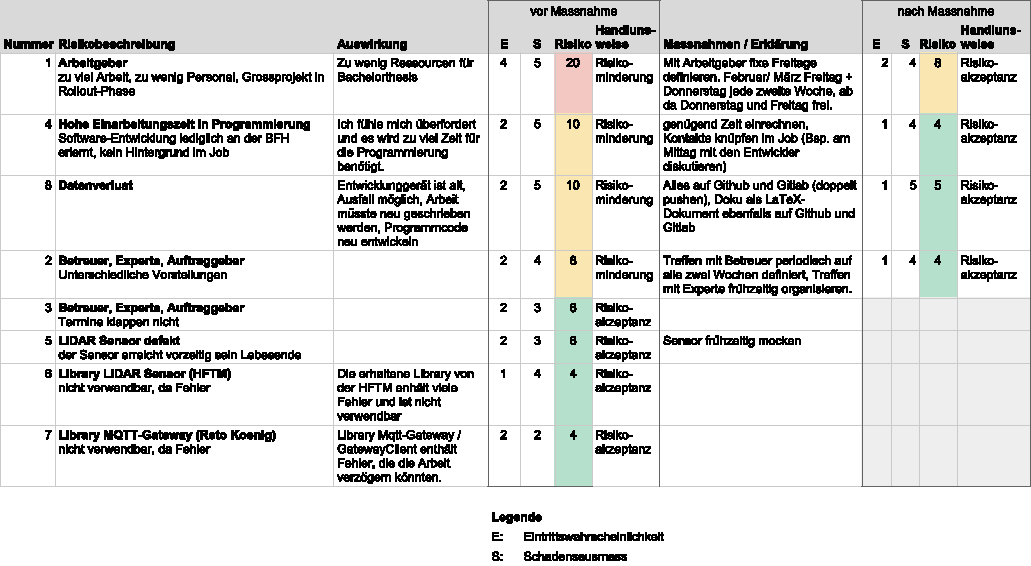
\includegraphics[width=1.0\textwidth]{img/risikoanalyse-tabelle.pdf}
	\caption{Risikoanalyse tabellarisch}
	\label{fig:risikoanalyse-tabelle}
\end{figure}
\begin{figure}[H]
	\centering
	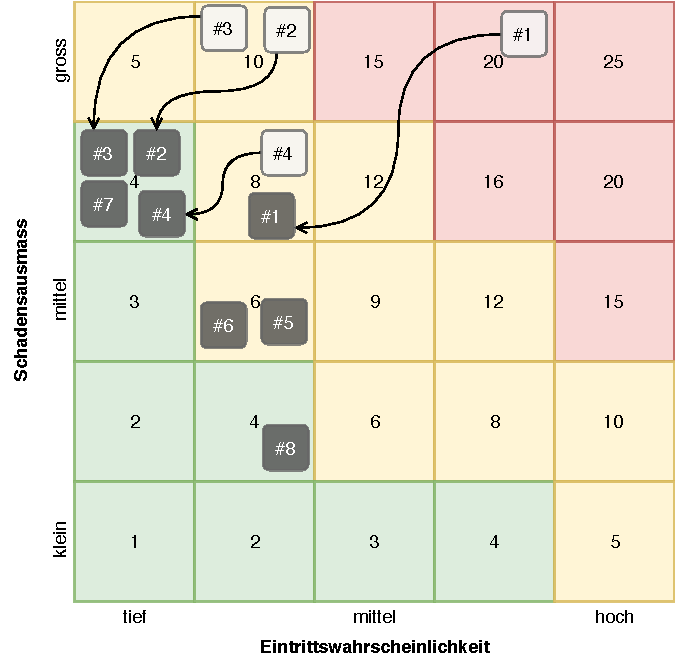
\includegraphics[width=0.5\textwidth]{img/risikoanalyse-matrix.pdf}
	\caption{Risikomatrix vor und nach ergreifen der Massnahmen}
	\label{fig:risikoanalyse-matrix}
\end{figure}


\section{Projektplan und Meilensteine}
\subsection{Meilensteine}
Als Meilensteine wurden lediglich die Termine mit fester Deadline festgelegt.
\begin{table}[H]
	\centering
	\begin{tabular}{llp{11cm}p{2cm}} \toprule
		\textbf{\#} 			& \textbf{Termin}	& \textbf{Beschreibung}	& \textbf{Erledigt}	\\ \midrule
		M1 & 08.03. & \textbf{Konzept verstanden} \newline Konzept verstehen vom GatewayClient, einfacher Service implementiert	& 08.03\\ \midrule
		M2 & 18.03. & \textbf{Referenzsetup fertiggestellt}\newline  Referenz-Setup mit 2x Service und 1x Servant, bereit um am Experten und Auftraggeber zu zeigen & 17.03.	\\ \midrule
		M3 & 01.06. & \textbf{Book und Poster}\newline  Plakat und Book fertig für die Abgabe & 01.06	\\ \midrule				
		M4 & 07.06. & \textbf{Dokumentation dem Auftraggeber vorlegen}\newline  Inhalt für Bericht soweit fertig, dass der Auftraggeber noch letzte Wünsche anbringen kann.& Feedback am 12.06.	\\ \midrule
		M5 & 14.06. & \textbf{Finish}\newline Bericht finalisiert, gedruckt, Code auf Github, Präsentation vorbereitet.	\\ \bottomrule
	\end{tabular}
	\caption{Meilensteine}
	\label{tab:meilensteine}
\end{table}

\subsection{Sprints}
Das Projekt wurde mit einer agilen Methode entwickelt, da zu Beginn der Arbeit nicht hundertprozentig klar war, wohin die Reise genau führt. Weil ich vom Job her bereits damit vertraut bin, wurde als Methode  Scrum in einer ,,Light''-Variante gewählt. Jedoch wurde auf die Toolschlacht, Sprint-Retrospektive und Co. verzichtet. Nachfolgend werden lediglich die auszuführenden Tasks aufgeführt:
\begin{figure}[H]
	\centering
	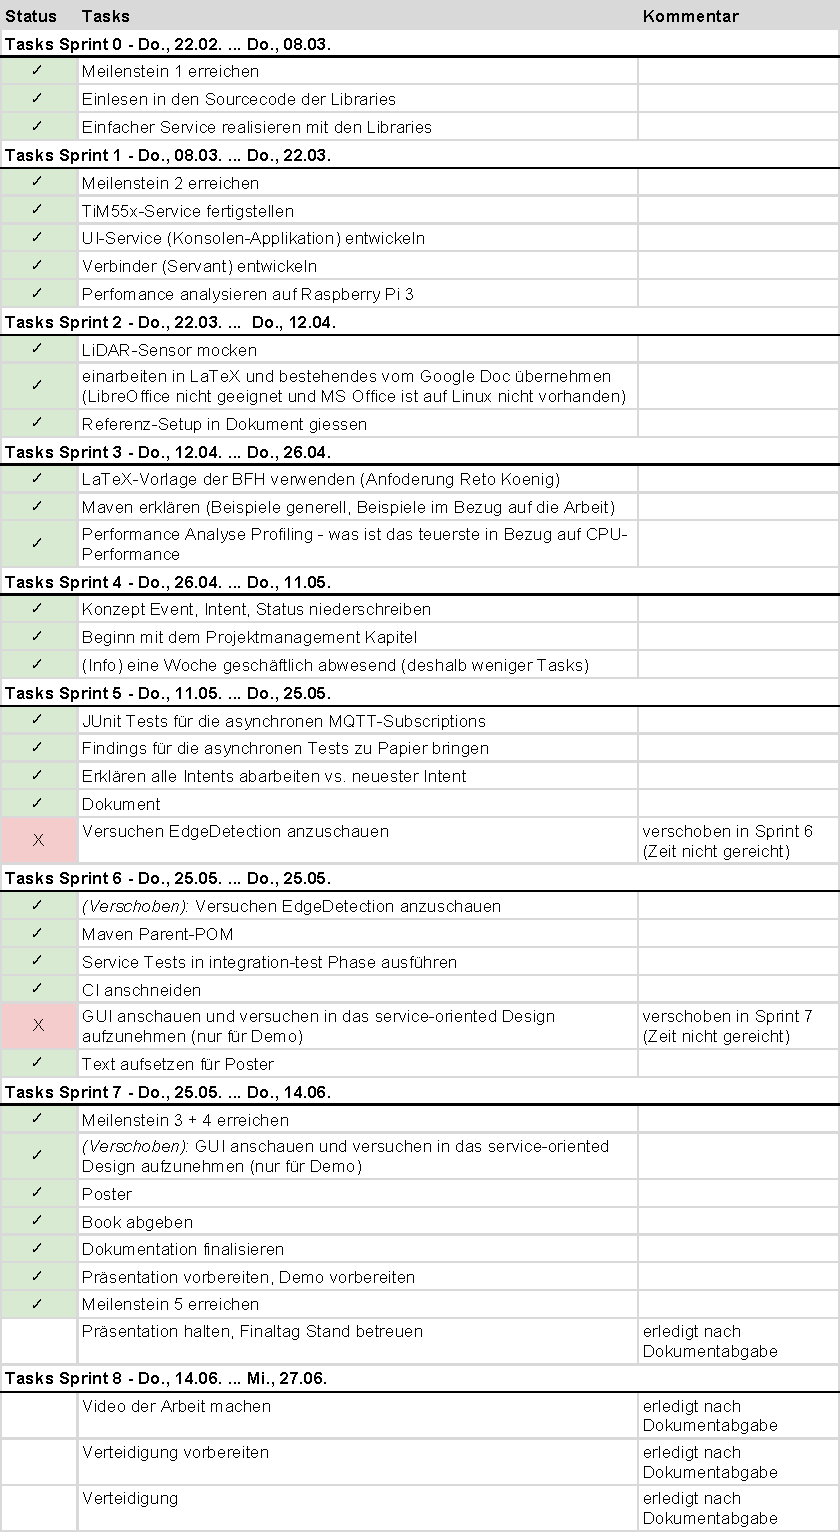
\includegraphics[width=0.7\textwidth]{img/sprintplanung.pdf}
	\caption{Sprintplanung tabellarisch}
	\label{fig:sprintplanung-tabelle}
\end{figure}

\subsection{fixe Termine}
\begin{table}[H]
	\centering
	\begin{tabular}{lll} \toprule
		\textbf{Datum} 			& \textbf{Termin Beschreibung}		& \textbf{Bemerkungen}		\\ \midrule
		Fr., 01.06.2018, 12:00		& Poster für Ausstellung 		& E-Mail an Heinz.Kipfer@bfh.ch	\\ \midrule
		Mo., 04.06.2018 		& Book - Freigabe Inhalte		& https://students.book.bfh.ch	\\ \midrule
		Mo., 11.06.2018 		& Book - Freigabe Layout		& https://students.book.bfh.ch	\\ \midrule
		Do., 14.06.2018, 20:00		& Abgabe Bericht			&  				\\ \midrule
		Fr., 15.06.2018, 10:40 - 10:55	& Präsentation Arbeit (Finaltag)	&  				\\ \midrule
		Fr., 22.06.2018			& Abgabe Film				& hochladen in Moodle		\\ \midrule
		Mi., 27.06.2018, 10:00 - 12:00	& Verteidigung				&				\\ \bottomrule
	\end{tabular}
	\caption{Fixe Termine während der Bachelorarbeit}
	\label{tab:fixeTermine}
\end{table}


\section{Meetings}
Mit dem Betreuer wurden zu Beginn dieser Arbeit die Meetings auf \underline{alle zwei Wochen} festgelegt. Bei Bedarf können Meetings auch kurzfristig stattfinden.
\subsection{Protokolle}
\subsubsection{Startvorlesung mit Herr Anrig (Mo., 19.02.2018)}
\begin{itemize}
	\item Aufgabenstellung erhalten
	\item Termine allgemein, alles auf Moodle
	\item Video ab diesem Semester Pflicht
	\item Eintrag im Book, Termin folgt (-> Entwurf: Mo., 04.06.2018, Freigabe: Mo., 11.06.2018)
	\item Plakat Vorlagen etc., Termin folgt (-> Fr., 01.06.2018, 12:00)
\end{itemize}

\subsubsection{Treffen mit Reto (Fr., 23.02.2018)}
\begin{itemize}
	\item Code für Java-GUI Software erhalten (Zip, Mail) -> Pushed auf https://gitlab.ti.bfh.ch/kilcm1/hftm-lidar
	\item Einführung in die Github Repos von knr1 (Reto Koenig) -> https://github.com/knr1?tab=repositories
	\item Festlegung der Treffen: alle zwei Wochen in Biel
\end{itemize}
Ziele: Lernbuch für HFTM (entweder in Doku integriert oder extern)


\subsubsection{Treffen mit Reto (Do., 08.03.2018)}
\begin{itemize}
	\item Erste Schritte mit dem GatewayClient gezeigt (LidarService).
\end{itemize}
nächste Schritte: Servant und kleiner UI-Service (Konsolen Interface) implementieren, danach Dokumentieren der ersten Erkenntnisse, Vorschlag für Treffen mit Experten (Dr. Joachim Wolfgang Kaltz)
\subsubsection{Treffen mit Experte (Mo., 19.03.2018)}
\begin{itemize}
	\item Vorhaben erklärt, HFTM und Studenten erläutert
	\item Experte ist einverstanden: die Arbeit könne gut ein Handbuch für die Studenten der HFTM sein. Kein Problem.
	\item Referenz-Setup mit den zwei Services und dem Servant gezeigt (Lidar, Console Client, Servant)
\end{itemize}
nächste Schritte: Weiteres Meeting mit Experte, Alain und Reto Mitte Mai.
\subsubsection{Treffen mit Reto (Do., 22.03.2018)}
nächste Schritte: Doku

\subsubsection{Treffen mit Reto und Alain (Do., 13.04.2018)}
\begin{itemize}
	\item Zugriff auf aktuellen Sourcecode vom Roboter erhalten (auf gitlab.com \cite{gitlab.com/solidus/hefei})
	\item Programmier-Niveau ist nicht sehr hoch und darf die Studenten nicht gleich überfordern. Java wird in 34 Lektionen vor dem Arbeiten am Robocup erst ausgebildet. Vorher haben die Meisten noch nie objektorientiert programmiert.
	\item Robi hat Intel i5-Basierter PC drauf (also doch kein Raspi) => ebenbürdig mit meinem Lenovo Yoga 2 Pro
\end{itemize}

\subsubsection{Treffen mit Reto (Do., 26.04.2018)}
\begin{itemize}
	\item Profiling angesprochen
	\item Alternativen mit "Kein Gluelayer"/Servant innerhalb einer Domain ansprechen, aber weiter wie bisher: zwischen jedem Service gibt es den Servant.
	\item Wenn es im Servant zu Ressourcen-Problemen kommt, verwenden wir eine andere Struktur als YAML/JSON (Bsp. Google's Protocol buffers)
\end{itemize}
nächste Schritte: Doku, Linien-Finder anschauen, Testing

\subsubsection{Treffen mit Reto (Do., 03.05.2018)}
\begin{itemize}
	\item Treffen mit Auftraggeber, Experten und Betreuer im Vorfeld nicht nötig (Mail 01. Mai 2018)
	\item Idee Services über Reference zusammenhängen, ohne die Daten durch den Servant zu schleusen, wenn kompatibel. Der Servant würde den entsprechenden Services das mitteilen.
	\item Zerreissen der "Library" für EdgeDetection, da Refactoring notwendig (Bsp. Naming der Koordinatensysteme Polar und Kartesisch)
\end{itemize}

\subsubsection{Treffen mit Reto (Do., 17.05.2018)}
\begin{itemize}
	\item Architekturbild (Datenfluss löschen und beim anderen Architekturbild bleiben)
	\item erklären weshalb nur der letzte LidarIntent genommen wird
	\item zwei Dokument-"Parts": Transition im Anhang und Setup/Grundlagen im Hauptteil (erklären weshalb)
	\item Pushen vom EdgeDetector - Stand heute, Reto schaut mal rein.
	\item Wording: 'Adapter' auf 'Service' ändern
	\item Annotations einführen für Contract / extends AValidator
	\item Umbenennung: Lidar-Service heisst TIM55x und EdgeDetector heisst 2DEdgeDetector
\end{itemize}

\subsubsection{Treffen mit Reto (Do., 31.05.2018)}
\begin{itemize}
	\item Poster Finalisiert
	\item Book mit einem Wortspiel ergänzen
\end{itemize}

\subsection{abgesagte Meetings}
\subsubsection{Treffen mit Reto und Alain (Do., 05.04.2018)}
abgesagt da Reto krank -> verschoben auf Fr., 13.04.2018, 09:00

\subsubsection{Treffen mit Reto (Do., 19.04.2018)}
abgesagt da Reto krank -> verschoben auf Do., 26.04.2018, 15:30

\section{Journal}
TODO: Bild vom Google Sheets einfügen am Schluss